\documentclass[twoside]{book}

% Packages required by doxygen
\usepackage{fixltx2e}
\usepackage{calc}
\usepackage{doxygen}
\usepackage[export]{adjustbox} % also loads graphicx
\usepackage{graphicx}
\usepackage[utf8]{inputenc}
\usepackage{makeidx}
\usepackage{multicol}
\usepackage{multirow}
\PassOptionsToPackage{warn}{textcomp}
\usepackage{textcomp}
\usepackage[nointegrals]{wasysym}
\usepackage[table]{xcolor}

% Font selection
\usepackage[T1]{fontenc}
\usepackage[scaled=.90]{helvet}
\usepackage{courier}
\usepackage{amssymb}
\usepackage{sectsty}
\renewcommand{\familydefault}{\sfdefault}
\allsectionsfont{%
  \fontseries{bc}\selectfont%
  \color{darkgray}%
}
\renewcommand{\DoxyLabelFont}{%
  \fontseries{bc}\selectfont%
  \color{darkgray}%
}
\newcommand{\+}{\discretionary{\mbox{\scriptsize$\hookleftarrow$}}{}{}}

% Page & text layout
\usepackage{geometry}
\geometry{%
  a4paper,%
  top=2.5cm,%
  bottom=2.5cm,%
  left=2.5cm,%
  right=2.5cm%
}
\tolerance=750
\hfuzz=15pt
\hbadness=750
\setlength{\emergencystretch}{15pt}
\setlength{\parindent}{0cm}
\setlength{\parskip}{3ex plus 2ex minus 2ex}
\makeatletter
\renewcommand{\paragraph}{%
  \@startsection{paragraph}{4}{0ex}{-1.0ex}{1.0ex}{%
    \normalfont\normalsize\bfseries\SS@parafont%
  }%
}
\renewcommand{\subparagraph}{%
  \@startsection{subparagraph}{5}{0ex}{-1.0ex}{1.0ex}{%
    \normalfont\normalsize\bfseries\SS@subparafont%
  }%
}
\makeatother

% Headers & footers
\usepackage{fancyhdr}
\pagestyle{fancyplain}
\fancyhead[LE]{\fancyplain{}{\bfseries\thepage}}
\fancyhead[CE]{\fancyplain{}{}}
\fancyhead[RE]{\fancyplain{}{\bfseries\leftmark}}
\fancyhead[LO]{\fancyplain{}{\bfseries\rightmark}}
\fancyhead[CO]{\fancyplain{}{}}
\fancyhead[RO]{\fancyplain{}{\bfseries\thepage}}
\fancyfoot[LE]{\fancyplain{}{}}
\fancyfoot[CE]{\fancyplain{}{}}
\fancyfoot[RE]{\fancyplain{}{\bfseries\scriptsize Generated by Doxygen }}
\fancyfoot[LO]{\fancyplain{}{\bfseries\scriptsize Generated by Doxygen }}
\fancyfoot[CO]{\fancyplain{}{}}
\fancyfoot[RO]{\fancyplain{}{}}
\renewcommand{\footrulewidth}{0.4pt}
\renewcommand{\chaptermark}[1]{%
  \markboth{#1}{}%
}
\renewcommand{\sectionmark}[1]{%
  \markright{\thesection\ #1}%
}

% Indices & bibliography
\usepackage{natbib}
\usepackage[titles]{tocloft}
\setcounter{tocdepth}{3}
\setcounter{secnumdepth}{5}
\makeindex

% Hyperlinks (required, but should be loaded last)
\usepackage{ifpdf}
\ifpdf
  \usepackage[pdftex,pagebackref=true]{hyperref}
\else
  \usepackage[ps2pdf,pagebackref=true]{hyperref}
\fi
\hypersetup{%
  colorlinks=true,%
  linkcolor=blue,%
  citecolor=blue,%
  unicode%
}

% Custom commands
\newcommand{\clearemptydoublepage}{%
  \newpage{\pagestyle{empty}\cleardoublepage}%
}

\usepackage{caption}
\captionsetup{labelsep=space,justification=centering,font={bf},singlelinecheck=off,skip=4pt,position=top}

%===== C O N T E N T S =====

\begin{document}

% Titlepage & ToC
\hypersetup{pageanchor=false,
             bookmarksnumbered=true,
             pdfencoding=unicode
            }
\pagenumbering{alph}
\begin{titlepage}
\vspace*{7cm}
\begin{center}%
{\Large Mininet }\\
\vspace*{1cm}
{\large Generated by Doxygen 1.8.12}\\
\end{center}
\end{titlepage}
\clearemptydoublepage
\pagenumbering{roman}
\tableofcontents
\clearemptydoublepage
\pagenumbering{arabic}
\hypersetup{pageanchor=true}

%--- Begin generated contents ---
\chapter{Hierarchical Index}
\section{Class Hierarchy}
This inheritance list is sorted roughly, but not completely, alphabetically\+:\begin{DoxyCompactList}
\item \contentsline{section}{mininet\+:\+:Backprop\+Params}{\pageref{structmininet_1_1_backprop_params}}{}
\item \contentsline{section}{mininet\+:\+:Dataset}{\pageref{classmininet_1_1_dataset}}{}
\item \contentsline{section}{mininet\+:\+:Layer}{\pageref{classmininet_1_1_layer}}{}
\begin{DoxyCompactList}
\item \contentsline{section}{mininet\+:\+:Hidden\+Layer}{\pageref{classmininet_1_1_hidden_layer}}{}
\begin{DoxyCompactList}
\item \contentsline{section}{mininet\+:\+:Re\+LU}{\pageref{classmininet_1_1_re_l_u}}{}
\end{DoxyCompactList}
\item \contentsline{section}{mininet\+:\+:Output\+Layer}{\pageref{classmininet_1_1_output_layer}}{}
\begin{DoxyCompactList}
\item \contentsline{section}{mininet\+:\+:Softmax}{\pageref{classmininet_1_1_softmax}}{}
\end{DoxyCompactList}
\end{DoxyCompactList}
\item \contentsline{section}{mininet\+:\+:Layer\+Params}{\pageref{structmininet_1_1_layer_params}}{}
\item \contentsline{section}{mininet\+:\+:Loss\+Functor}{\pageref{structmininet_1_1_loss_functor}}{}
\begin{DoxyCompactList}
\item \contentsline{section}{mininet\+:\+:Cross\+Entropy}{\pageref{structmininet_1_1_cross_entropy}}{}
\end{DoxyCompactList}
\item \contentsline{section}{mininet\+:\+:Network}{\pageref{classmininet_1_1_network}}{}
\item \contentsline{section}{mininet\+:\+:Trainer}{\pageref{classmininet_1_1_trainer}}{}
\begin{DoxyCompactList}
\item \contentsline{section}{mininet\+:\+:Backprop\+Trainer}{\pageref{classmininet_1_1_backprop_trainer}}{}
\end{DoxyCompactList}
\end{DoxyCompactList}

\chapter{Class Index}
\section{Class List}
Here are the classes, structs, unions and interfaces with brief descriptions\+:\begin{DoxyCompactList}
\item\contentsline{section}{\hyperlink{structmininet_1_1_backprop_params}{mininet\+::\+Backprop\+Params} }{\pageref{structmininet_1_1_backprop_params}}{}
\item\contentsline{section}{\hyperlink{classmininet_1_1_backprop_trainer}{mininet\+::\+Backprop\+Trainer} }{\pageref{classmininet_1_1_backprop_trainer}}{}
\item\contentsline{section}{\hyperlink{structmininet_1_1_cross_entropy}{mininet\+::\+Cross\+Entropy} }{\pageref{structmininet_1_1_cross_entropy}}{}
\item\contentsline{section}{\hyperlink{classmininet_1_1_dataset}{mininet\+::\+Dataset} }{\pageref{classmininet_1_1_dataset}}{}
\item\contentsline{section}{\hyperlink{structmininet_1_1_l2}{mininet\+::\+L2} }{\pageref{structmininet_1_1_l2}}{}
\item\contentsline{section}{\hyperlink{classmininet_1_1_layer}{mininet\+::\+Layer} }{\pageref{classmininet_1_1_layer}}{}
\item\contentsline{section}{\hyperlink{structmininet_1_1_layer_params}{mininet\+::\+Layer\+Params} }{\pageref{structmininet_1_1_layer_params}}{}
\item\contentsline{section}{\hyperlink{structmininet_1_1_loss_functor}{mininet\+::\+Loss\+Functor} }{\pageref{structmininet_1_1_loss_functor}}{}
\item\contentsline{section}{\hyperlink{classmininet_1_1_network}{mininet\+::\+Network} }{\pageref{classmininet_1_1_network}}{}
\item\contentsline{section}{\hyperlink{classmininet_1_1_re_l_u}{mininet\+::\+Re\+LU} }{\pageref{classmininet_1_1_re_l_u}}{}
\item\contentsline{section}{\hyperlink{classmininet_1_1_sigmoid}{mininet\+::\+Sigmoid} }{\pageref{classmininet_1_1_sigmoid}}{}
\item\contentsline{section}{\hyperlink{classmininet_1_1_softmax}{mininet\+::\+Softmax} }{\pageref{classmininet_1_1_softmax}}{}
\item\contentsline{section}{\hyperlink{classmininet_1_1_trainer}{mininet\+::\+Trainer} }{\pageref{classmininet_1_1_trainer}}{}
\end{DoxyCompactList}

\chapter{Class Documentation}
\hypertarget{structmininet_1_1_backprop_params}{}\section{mininet\+:\+:Backprop\+Params Struct Reference}
\label{structmininet_1_1_backprop_params}\index{mininet\+::\+Backprop\+Params@{mininet\+::\+Backprop\+Params}}
\subsection*{Public Attributes}
\begin{DoxyCompactItemize}
\item 
\hypertarget{structmininet_1_1_backprop_params_af4eee86c87c22531f2341de24ba90c86}{}\label{structmininet_1_1_backprop_params_af4eee86c87c22531f2341de24ba90c86} 
double {\bfseries max\+\_\+avg\+\_\+loss\+\_\+} = 1e-\/4
\item 
\hypertarget{structmininet_1_1_backprop_params_a89f75ef7b703abf69fde84f2df4e8648}{}\label{structmininet_1_1_backprop_params_a89f75ef7b703abf69fde84f2df4e8648} 
size\+\_\+t {\bfseries batch\+\_\+size\+\_\+} = 20
\item 
\hypertarget{structmininet_1_1_backprop_params_aa714c38be8deba2586ebb486a6f759dd}{}\label{structmininet_1_1_backprop_params_aa714c38be8deba2586ebb486a6f759dd} 
size\+\_\+t {\bfseries num\+\_\+iters\+\_\+per\+\_\+epoch\+\_\+} = 10
\item 
\hypertarget{structmininet_1_1_backprop_params_adf7d38efd1f9d8b12f69300c94b11bd6}{}\label{structmininet_1_1_backprop_params_adf7d38efd1f9d8b12f69300c94b11bd6} 
size\+\_\+t {\bfseries num\+\_\+epochs\+\_\+} = 10
\item 
\hypertarget{structmininet_1_1_backprop_params_ae7774867f9587f2f07a6fc8dc073585d}{}\label{structmininet_1_1_backprop_params_ae7774867f9587f2f07a6fc8dc073585d} 
double {\bfseries learning\+\_\+rate\+\_\+} = 0.\+1
\item 
\hypertarget{structmininet_1_1_backprop_params_abf7115d0cc8e9ae54d1aec6b2fc4ae21}{}\label{structmininet_1_1_backprop_params_abf7115d0cc8e9ae54d1aec6b2fc4ae21} 
double {\bfseries learning\+\_\+rate\+\_\+decay\+\_\+} = 0.\+5
\item 
\hypertarget{structmininet_1_1_backprop_params_a75dac35c45c55d6b5d8c18cee553c84b}{}\label{structmininet_1_1_backprop_params_a75dac35c45c55d6b5d8c18cee553c84b} 
double {\bfseries momentum\+\_\+} = 0.\+0
\item 
\hypertarget{structmininet_1_1_backprop_params_ae1f8124837580fe3b020213ed4f56772}{}\label{structmininet_1_1_backprop_params_ae1f8124837580fe3b020213ed4f56772} 
double {\bfseries weight\+\_\+decay\+\_\+} = 0.\+0
\end{DoxyCompactItemize}


\subsection{Detailed Description}


Definition at line 51 of file backprop\+\_\+params.\+h.



The documentation for this struct was generated from the following file\+:\begin{DoxyCompactItemize}
\item 
/\+Users/davidfridovichkeil/\+Documents/\+Developer/mininet/include/trainer/backprop\+\_\+params.\+h\end{DoxyCompactItemize}

\hypertarget{classmininet_1_1_backprop_trainer}{}\section{mininet\+:\+:Backprop\+Trainer Class Reference}
\label{classmininet_1_1_backprop_trainer}\index{mininet\+::\+Backprop\+Trainer@{mininet\+::\+Backprop\+Trainer}}
Inheritance diagram for mininet\+:\+:Backprop\+Trainer\+:\begin{figure}[H]
\begin{center}
\leavevmode
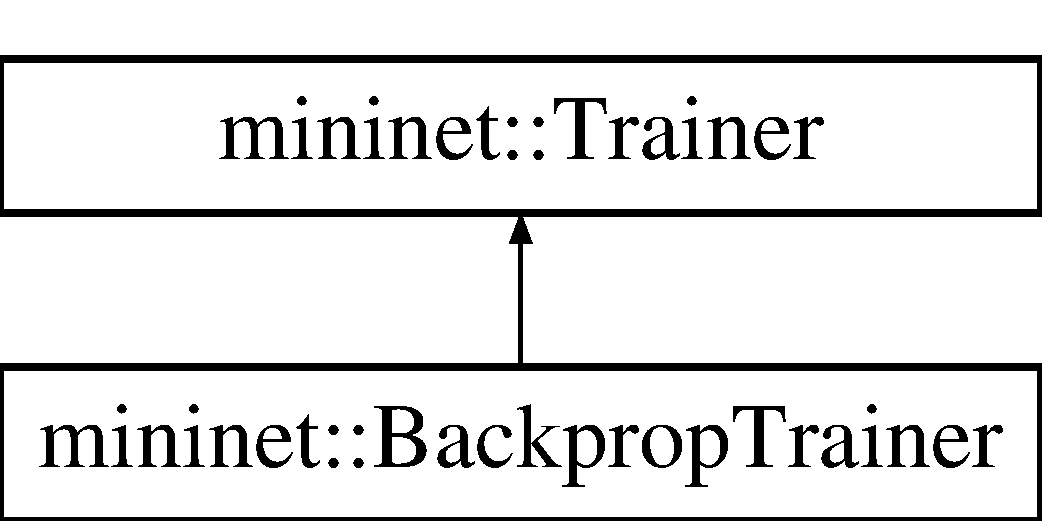
\includegraphics[height=2.000000cm]{classmininet_1_1_backprop_trainer}
\end{center}
\end{figure}
\subsection*{Public Member Functions}
\begin{DoxyCompactItemize}
\item 
\hypertarget{classmininet_1_1_backprop_trainer_a8cbf43d95c557921f1240b89e44b2da8}{}\label{classmininet_1_1_backprop_trainer_a8cbf43d95c557921f1240b89e44b2da8} 
{\bfseries Backprop\+Trainer} (const \hyperlink{classmininet_1_1_network}{Network} \&network, const \hyperlink{classmininet_1_1_dataset}{Dataset} \&dataset, const \hyperlink{structmininet_1_1_backprop_params}{Backprop\+Params} \&params)
\item 
\hypertarget{classmininet_1_1_backprop_trainer_a359c5b8e3d0a283aad185c2ba3d5ab0d}{}\label{classmininet_1_1_backprop_trainer_a359c5b8e3d0a283aad185c2ba3d5ab0d} 
double {\bfseries Train} ()
\end{DoxyCompactItemize}
\subsection*{Additional Inherited Members}


\subsection{Detailed Description}


Definition at line 52 of file backprop\+\_\+trainer.\+h.



The documentation for this class was generated from the following files\+:\begin{DoxyCompactItemize}
\item 
/\+Users/davidfridovichkeil/\+Documents/\+Developer/mininet/include/trainer/backprop\+\_\+trainer.\+h\item 
/\+Users/davidfridovichkeil/\+Documents/\+Developer/mininet/src/trainer/backprop\+\_\+trainer.\+cpp\end{DoxyCompactItemize}

\hypertarget{structmininet_1_1_cross_entropy}{}\section{mininet\+:\+:Cross\+Entropy Struct Reference}
\label{structmininet_1_1_cross_entropy}\index{mininet\+::\+Cross\+Entropy@{mininet\+::\+Cross\+Entropy}}
Inheritance diagram for mininet\+:\+:Cross\+Entropy\+:\begin{figure}[H]
\begin{center}
\leavevmode
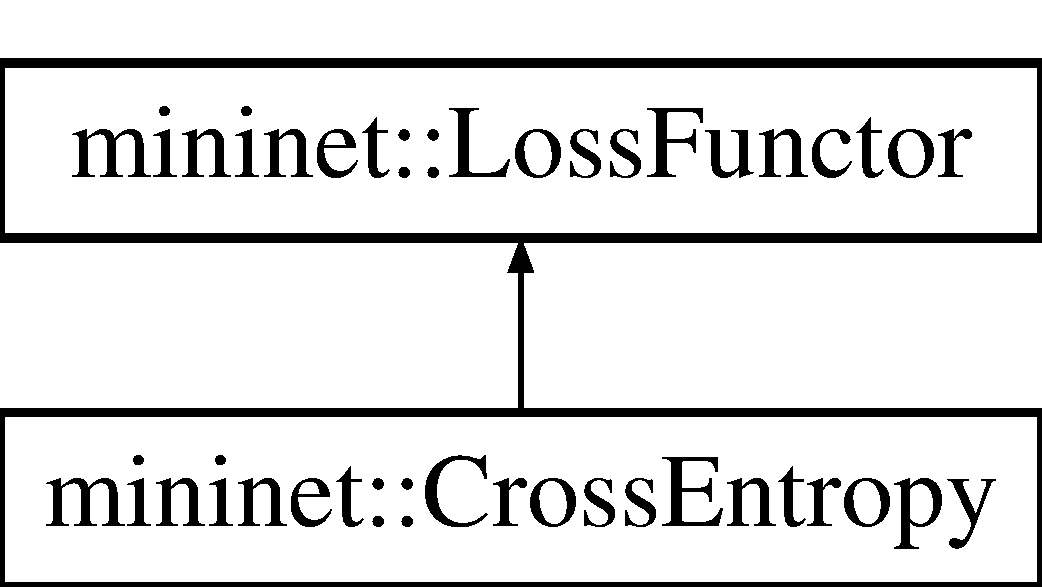
\includegraphics[height=2.000000cm]{structmininet_1_1_cross_entropy}
\end{center}
\end{figure}
\subsection*{Public Member Functions}
\begin{DoxyCompactItemize}
\item 
\hypertarget{structmininet_1_1_cross_entropy_af0d203db733d96a1c7eb4c6d0f7d51e5}{}\label{structmininet_1_1_cross_entropy_af0d203db733d96a1c7eb4c6d0f7d51e5} 
bool {\bfseries Evaluate} (const Vector\+Xd \&ground\+\_\+truth, const Vector\+Xd \&values, double \&loss, Vector\+Xd \&gradient) const
\end{DoxyCompactItemize}
\subsection*{Static Public Member Functions}
\begin{DoxyCompactItemize}
\item 
\hypertarget{structmininet_1_1_cross_entropy_ae736386755ec56b1adfaf643b1d114fa}{}\label{structmininet_1_1_cross_entropy_ae736386755ec56b1adfaf643b1d114fa} 
static Loss\+Functor\+::\+Ptr {\bfseries Create} ()
\end{DoxyCompactItemize}
\subsection*{Additional Inherited Members}


\subsection{Detailed Description}


Definition at line 54 of file cross\+\_\+entropy.\+h.



The documentation for this struct was generated from the following file\+:\begin{DoxyCompactItemize}
\item 
/\+Users/davidfridovichkeil/\+Documents/\+Developer/mininet/include/loss/cross\+\_\+entropy.\+h\end{DoxyCompactItemize}

\hypertarget{classmininet_1_1_dataset}{}\section{mininet\+:\+:Dataset Class Reference}
\label{classmininet_1_1_dataset}\index{mininet\+::\+Dataset@{mininet\+::\+Dataset}}
\subsection*{Public Member Functions}
\begin{DoxyCompactItemize}
\item 
\hypertarget{classmininet_1_1_dataset_a01534eefc85dfb4f68450516e595cf8b}{}\label{classmininet_1_1_dataset_a01534eefc85dfb4f68450516e595cf8b} 
{\bfseries Dataset} (const std\+::vector$<$ Vector\+Xd $>$ \&inputs, const std\+::vector$<$ Vector\+Xd $>$ \&outputs, double training\+\_\+fraction=0.\+65, bool normalize=true)
\item 
\hypertarget{classmininet_1_1_dataset_ad1b20aab3c1b240473810f9c1beabc0b}{}\label{classmininet_1_1_dataset_ad1b20aab3c1b240473810f9c1beabc0b} 
{\bfseries Dataset} (const std\+::vector$<$ Vector\+Xd $>$ \&training\+\_\+inputs, const std\+::vector$<$ Vector\+Xd $>$ \&training\+\_\+outputs, const std\+::vector$<$ Vector\+Xd $>$ \&validation\+\_\+inputs, const std\+::vector$<$ Vector\+Xd $>$ \&validation\+\_\+outputs, bool normalize=true)
\item 
\hypertarget{classmininet_1_1_dataset_a537e957564a9a742a41dc5da2cc64f9e}{}\label{classmininet_1_1_dataset_a537e957564a9a742a41dc5da2cc64f9e} 
bool {\bfseries Batch} (size\+\_\+t batch\+\_\+size, std\+::vector$<$ Vector\+Xd $>$ \&input\+\_\+samples, std\+::vector$<$ Vector\+Xd $>$ \&output\+\_\+samples)
\item 
\hypertarget{classmininet_1_1_dataset_aa65cbe648ae6ccb85261c2230526f254}{}\label{classmininet_1_1_dataset_aa65cbe648ae6ccb85261c2230526f254} 
const std\+::vector$<$ Vector\+Xd $>$ \& {\bfseries Validation\+Inputs} () const
\item 
\hypertarget{classmininet_1_1_dataset_a027524a596c8cd557c7a54e7c189505c}{}\label{classmininet_1_1_dataset_a027524a596c8cd557c7a54e7c189505c} 
const std\+::vector$<$ Vector\+Xd $>$ \& {\bfseries Validation\+Outputs} () const
\end{DoxyCompactItemize}


\subsection{Detailed Description}


Definition at line 55 of file dataset.\+h.



The documentation for this class was generated from the following files\+:\begin{DoxyCompactItemize}
\item 
/\+Users/davidfridovichkeil/\+Documents/\+Developer/mininet/include/dataset/dataset.\+h\item 
/\+Users/davidfridovichkeil/\+Documents/\+Developer/mininet/src/dataset/dataset.\+cpp\end{DoxyCompactItemize}

\hypertarget{classmininet_1_1_hidden_layer}{}\section{mininet\+:\+:Hidden\+Layer Class Reference}
\label{classmininet_1_1_hidden_layer}\index{mininet\+::\+Hidden\+Layer@{mininet\+::\+Hidden\+Layer}}
Inheritance diagram for mininet\+:\+:Hidden\+Layer\+:\begin{figure}[H]
\begin{center}
\leavevmode
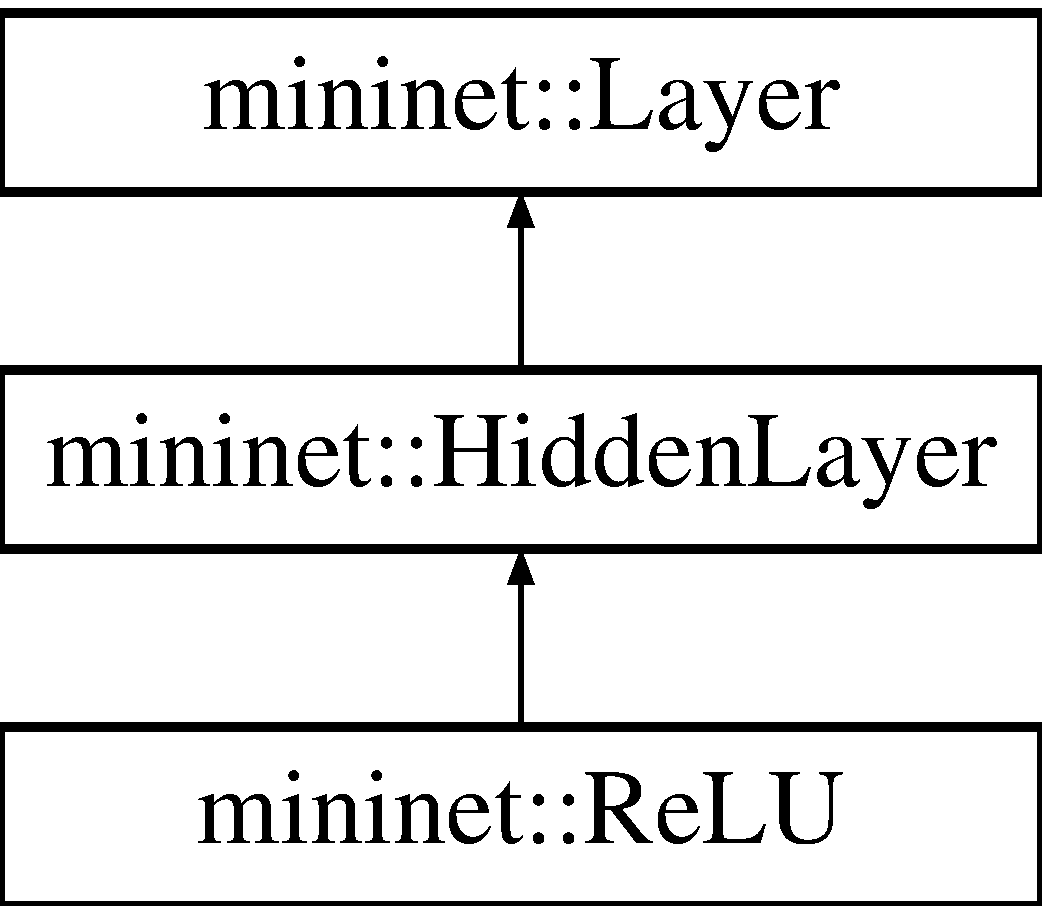
\includegraphics[height=3.000000cm]{classmininet_1_1_hidden_layer}
\end{center}
\end{figure}
\subsection*{Public Types}
\begin{DoxyCompactItemize}
\item 
\hypertarget{classmininet_1_1_hidden_layer_a2be764b9978a6288b26b56f40ee9bfe4}{}\label{classmininet_1_1_hidden_layer_a2be764b9978a6288b26b56f40ee9bfe4} 
typedef std\+::shared\+\_\+ptr$<$ \hyperlink{classmininet_1_1_hidden_layer}{Hidden\+Layer} $>$ {\bfseries Ptr}
\item 
\hypertarget{classmininet_1_1_hidden_layer_a0cc783f56aa7d749862dfc4cc60f1bce}{}\label{classmininet_1_1_hidden_layer_a0cc783f56aa7d749862dfc4cc60f1bce} 
typedef std\+::shared\+\_\+ptr$<$ const \hyperlink{classmininet_1_1_hidden_layer}{Hidden\+Layer} $>$ {\bfseries Const\+Ptr}
\end{DoxyCompactItemize}
\subsection*{Public Member Functions}
\begin{DoxyCompactItemize}
\item 
\hypertarget{classmininet_1_1_hidden_layer_ae7f168cf012746112311407332886b15}{}\label{classmininet_1_1_hidden_layer_ae7f168cf012746112311407332886b15} 
{\bfseries Hidden\+Layer} (size\+\_\+t input\+\_\+size, size\+\_\+t output\+\_\+size)
\item 
\hypertarget{classmininet_1_1_hidden_layer_a8c2915edd9ea952a6ae278ebdee99c92}{}\label{classmininet_1_1_hidden_layer_a8c2915edd9ea952a6ae278ebdee99c92} 
virtual void {\bfseries Backward} (const Vector\+Xd \&output, const Vector\+Xd \&upstream\+\_\+gammas, Vector\+Xd \&gammas, Vector\+Xd \&deltas) const =0
\end{DoxyCompactItemize}
\subsection*{Additional Inherited Members}


\subsection{Detailed Description}


Definition at line 52 of file hidden\+\_\+layer.\+h.



The documentation for this class was generated from the following file\+:\begin{DoxyCompactItemize}
\item 
/\+Users/davidfridovichkeil/\+Documents/\+Developer/mininet/include/layer/hidden\+\_\+layer.\+h\end{DoxyCompactItemize}

\hypertarget{classmininet_1_1_layer}{}\section{mininet\+:\+:Layer Class Reference}
\label{classmininet_1_1_layer}\index{mininet\+::\+Layer@{mininet\+::\+Layer}}
Inheritance diagram for mininet\+:\+:Layer\+:\begin{figure}[H]
\begin{center}
\leavevmode
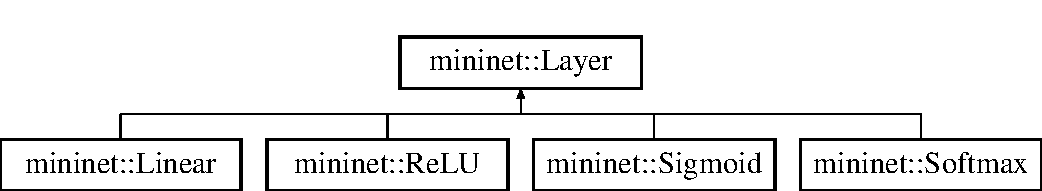
\includegraphics[height=2.000000cm]{classmininet_1_1_layer}
\end{center}
\end{figure}
\subsection*{Public Types}
\begin{DoxyCompactItemize}
\item 
\hypertarget{classmininet_1_1_layer_a16a0db407855771f9b7465ff1551f8cb}{}\label{classmininet_1_1_layer_a16a0db407855771f9b7465ff1551f8cb} 
typedef std\+::shared\+\_\+ptr$<$ \hyperlink{classmininet_1_1_layer}{Layer} $>$ {\bfseries Ptr}
\item 
\hypertarget{classmininet_1_1_layer_a788af6d5c8e9588770e6717776621201}{}\label{classmininet_1_1_layer_a788af6d5c8e9588770e6717776621201} 
typedef std\+::shared\+\_\+ptr$<$ const \hyperlink{classmininet_1_1_layer}{Layer} $>$ {\bfseries Const\+Ptr}
\end{DoxyCompactItemize}
\subsection*{Public Member Functions}
\begin{DoxyCompactItemize}
\item 
\hypertarget{classmininet_1_1_layer_aed25482510bfaf3ca2fbea9897ddb352}{}\label{classmininet_1_1_layer_aed25482510bfaf3ca2fbea9897ddb352} 
{\bfseries Layer} (size\+\_\+t input\+\_\+size, size\+\_\+t output\+\_\+size)
\item 
\hypertarget{classmininet_1_1_layer_a1e4d5bfdc7e78035d185e4a1a690d53b}{}\label{classmininet_1_1_layer_a1e4d5bfdc7e78035d185e4a1a690d53b} 
size\+\_\+t {\bfseries Input\+Size} () const
\item 
\hypertarget{classmininet_1_1_layer_a57a99b9937ce76a1a6e57903f308aba4}{}\label{classmininet_1_1_layer_a57a99b9937ce76a1a6e57903f308aba4} 
size\+\_\+t {\bfseries Output\+Size} () const
\item 
\hypertarget{classmininet_1_1_layer_a294ed3ba99229b383cf0486a5bbc67bb}{}\label{classmininet_1_1_layer_a294ed3ba99229b383cf0486a5bbc67bb} 
const Matrix\+Xd \& {\bfseries Immutable\+Weights} () const
\item 
\hypertarget{classmininet_1_1_layer_a2b45d5d75030e782f43ff46972d471f8}{}\label{classmininet_1_1_layer_a2b45d5d75030e782f43ff46972d471f8} 
void {\bfseries Update\+Weights} (const Matrix\+Xd \&derivatives, double learning\+\_\+rate, double momentum=0.\+0, double decay=0.\+0)
\item 
\hypertarget{classmininet_1_1_layer_a20738f447572a1fa759decae8913814f}{}\label{classmininet_1_1_layer_a20738f447572a1fa759decae8913814f} 
void {\bfseries Perturb\+Weight} (size\+\_\+t ii, size\+\_\+t jj, double amount)
\item 
\hypertarget{classmininet_1_1_layer_a933df55c92eb813d3e69e9ecfa42dfa6}{}\label{classmininet_1_1_layer_a933df55c92eb813d3e69e9ecfa42dfa6} 
virtual void {\bfseries Forward} (const Vector\+Xd \&input, Vector\+Xd \&output) const =0
\item 
\hypertarget{classmininet_1_1_layer_adcb8e5bd70a76f479c9448def491576f}{}\label{classmininet_1_1_layer_adcb8e5bd70a76f479c9448def491576f} 
virtual void {\bfseries Backward} (const Vector\+Xd \&output, const Vector\+Xd \&upstream\+\_\+gammas, Vector\+Xd \&gammas, Vector\+Xd \&deltas) const =0
\item 
\hypertarget{classmininet_1_1_layer_a979f63fe1e0d4b907b6a7adb7767b75e}{}\label{classmininet_1_1_layer_a979f63fe1e0d4b907b6a7adb7767b75e} 
virtual double {\bfseries Backward} (const Loss\+Functor\+::\+Const\+Ptr \&loss, const Vector\+Xd \&ground\+\_\+truth, const Vector\+Xd \&output, Vector\+Xd \&gammas, Vector\+Xd \&deltas) const =0
\end{DoxyCompactItemize}
\subsection*{Protected Attributes}
\begin{DoxyCompactItemize}
\item 
\hypertarget{classmininet_1_1_layer_a9be2fab58f1a70c74b84c6fed4eac6c9}{}\label{classmininet_1_1_layer_a9be2fab58f1a70c74b84c6fed4eac6c9} 
Matrix\+Xd {\bfseries weights\+\_\+}
\item 
\hypertarget{classmininet_1_1_layer_a36fb12285a038b6d1afefe9ea29946dc}{}\label{classmininet_1_1_layer_a36fb12285a038b6d1afefe9ea29946dc} 
Matrix\+Xd {\bfseries weight\+\_\+changes\+\_\+}
\end{DoxyCompactItemize}


\subsection{Detailed Description}


Definition at line 54 of file layer.\+h.



The documentation for this class was generated from the following files\+:\begin{DoxyCompactItemize}
\item 
/\+Users/davidfridovichkeil/\+Documents/\+Developer/mininet/include/layer/layer.\+h\item 
/\+Users/davidfridovichkeil/\+Documents/\+Developer/mininet/src/layer/layer.\+cpp\end{DoxyCompactItemize}

\hypertarget{structmininet_1_1_layer_params}{}\section{mininet\+:\+:Layer\+Params Struct Reference}
\label{structmininet_1_1_layer_params}\index{mininet\+::\+Layer\+Params@{mininet\+::\+Layer\+Params}}
\subsection*{Public Attributes}
\begin{DoxyCompactItemize}
\item 
\hypertarget{structmininet_1_1_layer_params_afe73b1c539544ca3e280d3e5dd222007}{}\label{structmininet_1_1_layer_params_afe73b1c539544ca3e280d3e5dd222007} 
Layer\+Type {\bfseries type\+\_\+} = R\+E\+LU
\item 
\hypertarget{structmininet_1_1_layer_params_af572460aed17881f265fefec48bdba76}{}\label{structmininet_1_1_layer_params_af572460aed17881f265fefec48bdba76} 
size\+\_\+t {\bfseries input\+\_\+size\+\_\+} = 10
\item 
\hypertarget{structmininet_1_1_layer_params_ab3c57b124160125c98e5a960cf653efc}{}\label{structmininet_1_1_layer_params_ab3c57b124160125c98e5a960cf653efc} 
size\+\_\+t {\bfseries output\+\_\+size\+\_\+} = 10
\end{DoxyCompactItemize}


\subsection{Detailed Description}


Definition at line 51 of file layer\+\_\+params.\+h.



The documentation for this struct was generated from the following file\+:\begin{DoxyCompactItemize}
\item 
/\+Users/davidfridovichkeil/\+Documents/\+Developer/mininet/include/layer/layer\+\_\+params.\+h\end{DoxyCompactItemize}

\hypertarget{structmininet_1_1_loss_functor}{}\section{mininet\+:\+:Loss\+Functor Struct Reference}
\label{structmininet_1_1_loss_functor}\index{mininet\+::\+Loss\+Functor@{mininet\+::\+Loss\+Functor}}
Inheritance diagram for mininet\+:\+:Loss\+Functor\+:\begin{figure}[H]
\begin{center}
\leavevmode
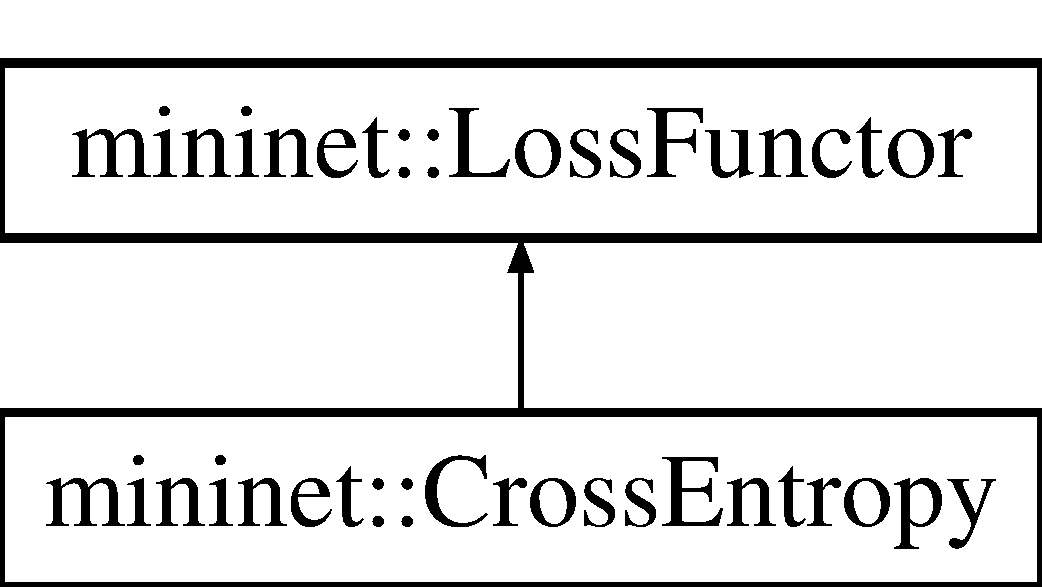
\includegraphics[height=2.000000cm]{structmininet_1_1_loss_functor}
\end{center}
\end{figure}
\subsection*{Public Types}
\begin{DoxyCompactItemize}
\item 
\hypertarget{structmininet_1_1_loss_functor_a83844446699ed7e2acd3ded37dcdea30}{}\label{structmininet_1_1_loss_functor_a83844446699ed7e2acd3ded37dcdea30} 
typedef std\+::shared\+\_\+ptr$<$ \hyperlink{structmininet_1_1_loss_functor}{Loss\+Functor} $>$ {\bfseries Ptr}
\item 
\hypertarget{structmininet_1_1_loss_functor_a364ddba572476df7162f90d0b1f3edc0}{}\label{structmininet_1_1_loss_functor_a364ddba572476df7162f90d0b1f3edc0} 
typedef std\+::shared\+\_\+ptr$<$ const \hyperlink{structmininet_1_1_loss_functor}{Loss\+Functor} $>$ {\bfseries Const\+Ptr}
\end{DoxyCompactItemize}
\subsection*{Public Member Functions}
\begin{DoxyCompactItemize}
\item 
\hypertarget{structmininet_1_1_loss_functor_ae802e879737d401de2b08acabe976eb8}{}\label{structmininet_1_1_loss_functor_ae802e879737d401de2b08acabe976eb8} 
virtual bool {\bfseries Evaluate} (const Vector\+Xd \&ground\+\_\+truth, const Vector\+Xd \&values, double \&loss, Vector\+Xd \&gradient) const =0
\end{DoxyCompactItemize}


\subsection{Detailed Description}


Definition at line 53 of file loss\+\_\+functor.\+h.



The documentation for this struct was generated from the following file\+:\begin{DoxyCompactItemize}
\item 
/\+Users/davidfridovichkeil/\+Documents/\+Developer/mininet/include/loss/loss\+\_\+functor.\+h\end{DoxyCompactItemize}

\hypertarget{classmininet_1_1_network}{}\section{mininet\+:\+:Network Class Reference}
\label{classmininet_1_1_network}\index{mininet\+::\+Network@{mininet\+::\+Network}}
\subsection*{Public Member Functions}
\begin{DoxyCompactItemize}
\item 
\hypertarget{classmininet_1_1_network_acf2c102c6f79c152380124af7b327b89}{}\label{classmininet_1_1_network_acf2c102c6f79c152380124af7b327b89} 
{\bfseries Network} (std\+::vector$<$ \hyperlink{structmininet_1_1_layer_params}{Layer\+Params} $>$ params, const Loss\+Functor\+::\+Const\+Ptr \&loss)
\item 
\hypertarget{classmininet_1_1_network_a56fe1d7f1daf3433c9f0d5df408b4800}{}\label{classmininet_1_1_network_a56fe1d7f1daf3433c9f0d5df408b4800} 
void {\bfseries operator()} (const Vector\+Xd \&input, Vector\+Xd \&output) const
\item 
\hypertarget{classmininet_1_1_network_ae76628cf7258aa0b8d0ee147e580623e}{}\label{classmininet_1_1_network_ae76628cf7258aa0b8d0ee147e580623e} 
double {\bfseries Loss} (const std\+::vector$<$ Vector\+Xd $>$ \&inputs, const std\+::vector$<$ Vector\+Xd $>$ \&ground\+\_\+truths) const
\item 
\hypertarget{classmininet_1_1_network_a52d7bf3f7a6ff4ca2d2fe93758b48cc0}{}\label{classmininet_1_1_network_a52d7bf3f7a6ff4ca2d2fe93758b48cc0} 
double {\bfseries Run\+Batch} (const std\+::vector$<$ Vector\+Xd $>$ \&batch, const std\+::vector$<$ Vector\+Xd $>$ \&ground\+\_\+truth, std\+::vector$<$ Matrix\+Xd $>$ \&derivatives) const
\item 
\hypertarget{classmininet_1_1_network_a09c5c7f9617732fa35308e0218e06ec8}{}\label{classmininet_1_1_network_a09c5c7f9617732fa35308e0218e06ec8} 
void {\bfseries Update\+Weights} (const std\+::vector$<$ Matrix\+Xd $>$ \&derivatives, double step\+\_\+size)
\item 
\hypertarget{classmininet_1_1_network_a3b1a8593348f1e0aa1a4a1457d3d6ab2}{}\label{classmininet_1_1_network_a3b1a8593348f1e0aa1a4a1457d3d6ab2} 
void {\bfseries Perturb\+Weight} (size\+\_\+t layer\+\_\+number, size\+\_\+t ii, size\+\_\+t jj, double amount)
\end{DoxyCompactItemize}


\subsection{Detailed Description}


Definition at line 57 of file network.\+h.



The documentation for this class was generated from the following files\+:\begin{DoxyCompactItemize}
\item 
/\+Users/davidfridovichkeil/\+Documents/\+Developer/mininet/include/net/network.\+h\item 
/\+Users/davidfridovichkeil/\+Documents/\+Developer/mininet/src/net/network.\+cpp\end{DoxyCompactItemize}

\hypertarget{classmininet_1_1_output_layer}{}\section{mininet\+:\+:Output\+Layer Class Reference}
\label{classmininet_1_1_output_layer}\index{mininet\+::\+Output\+Layer@{mininet\+::\+Output\+Layer}}
Inheritance diagram for mininet\+:\+:Output\+Layer\+:\begin{figure}[H]
\begin{center}
\leavevmode
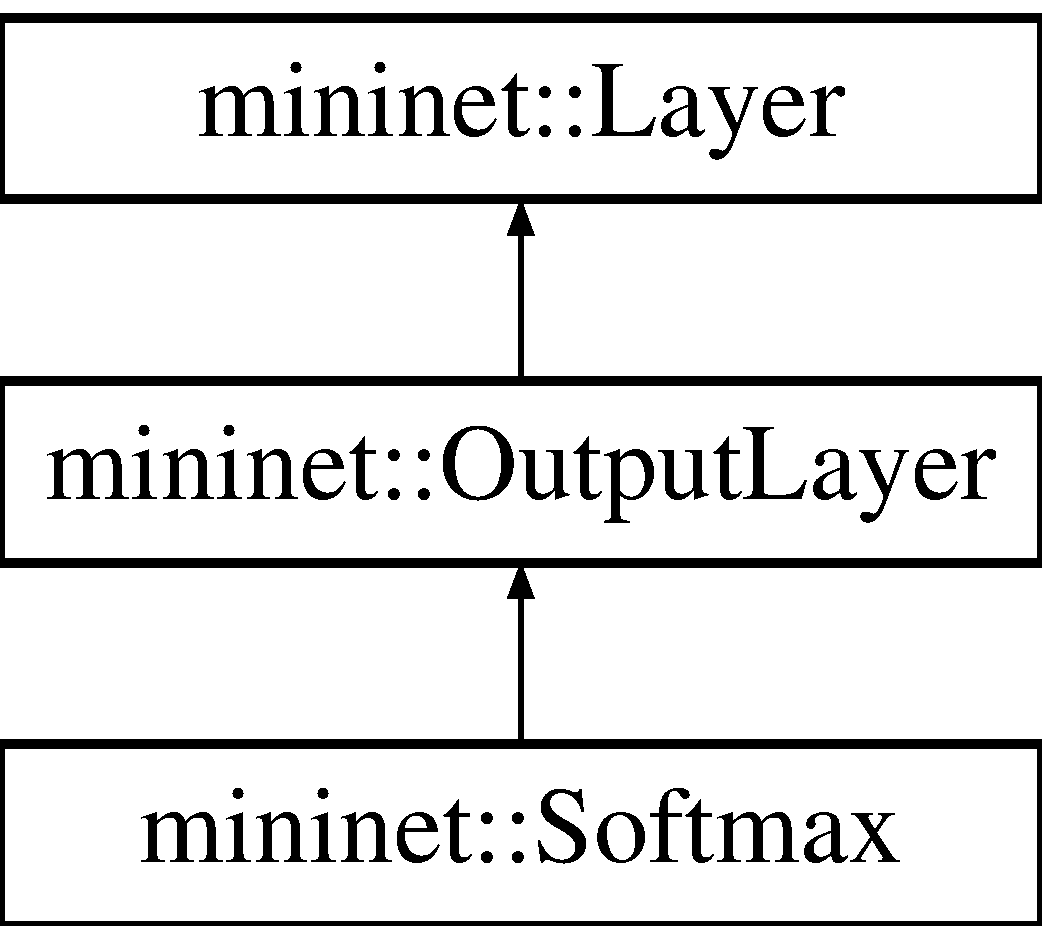
\includegraphics[height=3.000000cm]{classmininet_1_1_output_layer}
\end{center}
\end{figure}
\subsection*{Public Types}
\begin{DoxyCompactItemize}
\item 
\hypertarget{classmininet_1_1_output_layer_acc7e50578531001eb4e03468f6a55eac}{}\label{classmininet_1_1_output_layer_acc7e50578531001eb4e03468f6a55eac} 
typedef std\+::shared\+\_\+ptr$<$ \hyperlink{classmininet_1_1_output_layer}{Output\+Layer} $>$ {\bfseries Ptr}
\item 
\hypertarget{classmininet_1_1_output_layer_a96657e2d32023e3025e55c3dffc4bca2}{}\label{classmininet_1_1_output_layer_a96657e2d32023e3025e55c3dffc4bca2} 
typedef std\+::shared\+\_\+ptr$<$ const \hyperlink{classmininet_1_1_output_layer}{Output\+Layer} $>$ {\bfseries Const\+Ptr}
\end{DoxyCompactItemize}
\subsection*{Public Member Functions}
\begin{DoxyCompactItemize}
\item 
\hypertarget{classmininet_1_1_output_layer_abe454b2360d589f5ff00daa3cf699d91}{}\label{classmininet_1_1_output_layer_abe454b2360d589f5ff00daa3cf699d91} 
{\bfseries Output\+Layer} (size\+\_\+t input\+\_\+size, size\+\_\+t output\+\_\+size)
\item 
\hypertarget{classmininet_1_1_output_layer_a8b863c7c620886f745578a58e03c4fb9}{}\label{classmininet_1_1_output_layer_a8b863c7c620886f745578a58e03c4fb9} 
virtual double {\bfseries Backward} (const Loss\+Functor\+::\+Const\+Ptr \&loss, const Vector\+Xd \&ground\+\_\+truth, const Vector\+Xd \&output, Vector\+Xd \&gammas, Vector\+Xd \&deltas) const =0
\end{DoxyCompactItemize}
\subsection*{Additional Inherited Members}


\subsection{Detailed Description}


Definition at line 53 of file output\+\_\+layer.\+h.



The documentation for this class was generated from the following file\+:\begin{DoxyCompactItemize}
\item 
/\+Users/davidfridovichkeil/\+Documents/\+Developer/mininet/include/layer/output\+\_\+layer.\+h\end{DoxyCompactItemize}

\hypertarget{classmininet_1_1_re_l_u}{}\section{mininet\+:\+:Re\+LU Class Reference}
\label{classmininet_1_1_re_l_u}\index{mininet\+::\+Re\+LU@{mininet\+::\+Re\+LU}}
Inheritance diagram for mininet\+:\+:Re\+LU\+:\begin{figure}[H]
\begin{center}
\leavevmode
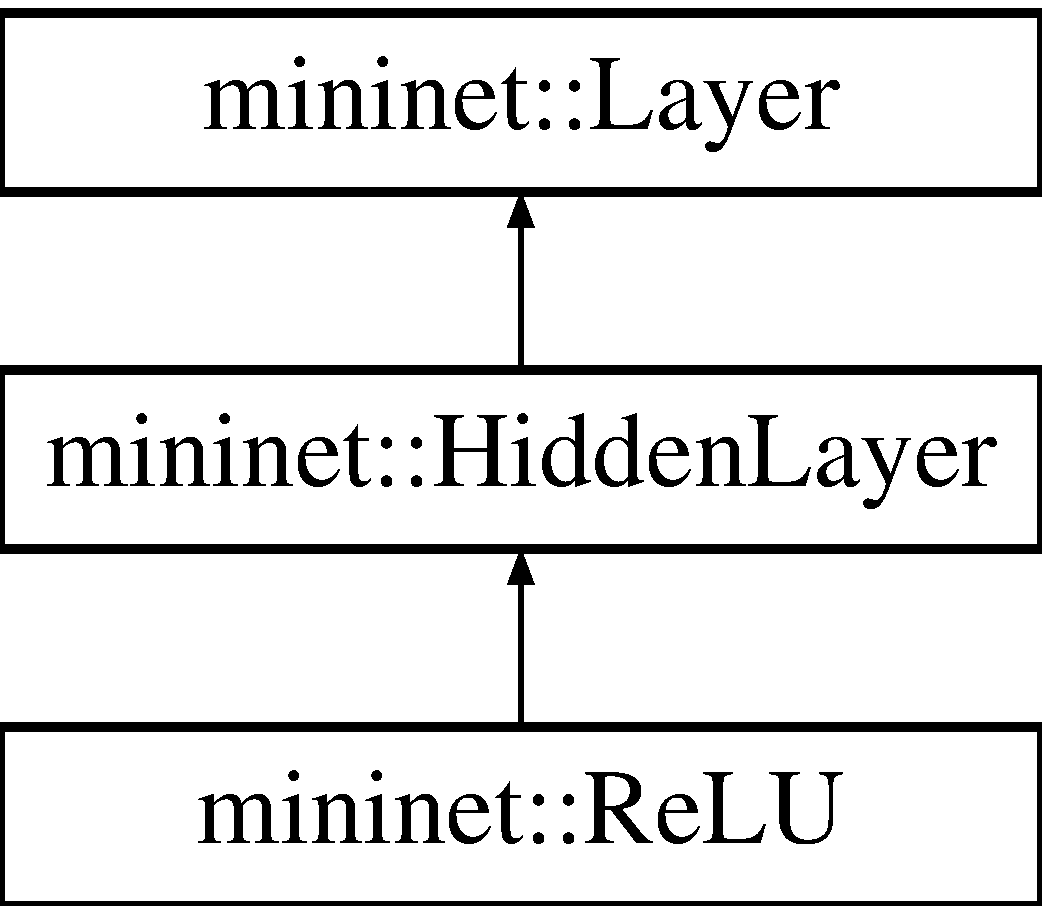
\includegraphics[height=2.000000cm]{classmininet_1_1_re_l_u}
\end{center}
\end{figure}
\subsection*{Public Member Functions}
\begin{DoxyCompactItemize}
\item 
\hypertarget{classmininet_1_1_re_l_u_a735805e56b2d230e1b48ac0e02487c40}{}\label{classmininet_1_1_re_l_u_a735805e56b2d230e1b48ac0e02487c40} 
void {\bfseries Forward} (const Vector\+Xd \&input, Vector\+Xd \&output) const
\item 
\hypertarget{classmininet_1_1_re_l_u_a01bb8ec3b01d9f8dfb175c62490f109e}{}\label{classmininet_1_1_re_l_u_a01bb8ec3b01d9f8dfb175c62490f109e} 
void {\bfseries Backward} (const Vector\+Xd \&output, const Vector\+Xd \&upstream\+\_\+gammas, Vector\+Xd \&gammas, Vector\+Xd \&deltas) const
\item 
\hypertarget{classmininet_1_1_re_l_u_ad7ce7471c4a9fea71e2f4e68051f939d}{}\label{classmininet_1_1_re_l_u_ad7ce7471c4a9fea71e2f4e68051f939d} 
double {\bfseries Backward} (const Loss\+Functor\+::\+Const\+Ptr \&loss, const Vector\+Xd \&ground\+\_\+truth, const Vector\+Xd \&output, Vector\+Xd \&gammas, Vector\+Xd \&deltas) const
\end{DoxyCompactItemize}
\subsection*{Static Public Member Functions}
\begin{DoxyCompactItemize}
\item 
\hypertarget{classmininet_1_1_re_l_u_a1d9e8079466ab4a85bb01894877045a6}{}\label{classmininet_1_1_re_l_u_a1d9e8079466ab4a85bb01894877045a6} 
static Layer\+::\+Ptr {\bfseries Create} (size\+\_\+t input\+\_\+size, size\+\_\+t output\+\_\+size)
\end{DoxyCompactItemize}
\subsection*{Additional Inherited Members}


\subsection{Detailed Description}


Definition at line 52 of file relu.\+h.



The documentation for this class was generated from the following files\+:\begin{DoxyCompactItemize}
\item 
/\+Users/davidfridovichkeil/\+Documents/\+Developer/mininet/include/layer/relu.\+h\item 
/\+Users/davidfridovichkeil/\+Documents/\+Developer/mininet/src/layer/relu.\+cpp\end{DoxyCompactItemize}

\hypertarget{classmininet_1_1_softmax}{}\section{mininet\+:\+:Softmax Class Reference}
\label{classmininet_1_1_softmax}\index{mininet\+::\+Softmax@{mininet\+::\+Softmax}}
Inheritance diagram for mininet\+:\+:Softmax\+:\begin{figure}[H]
\begin{center}
\leavevmode
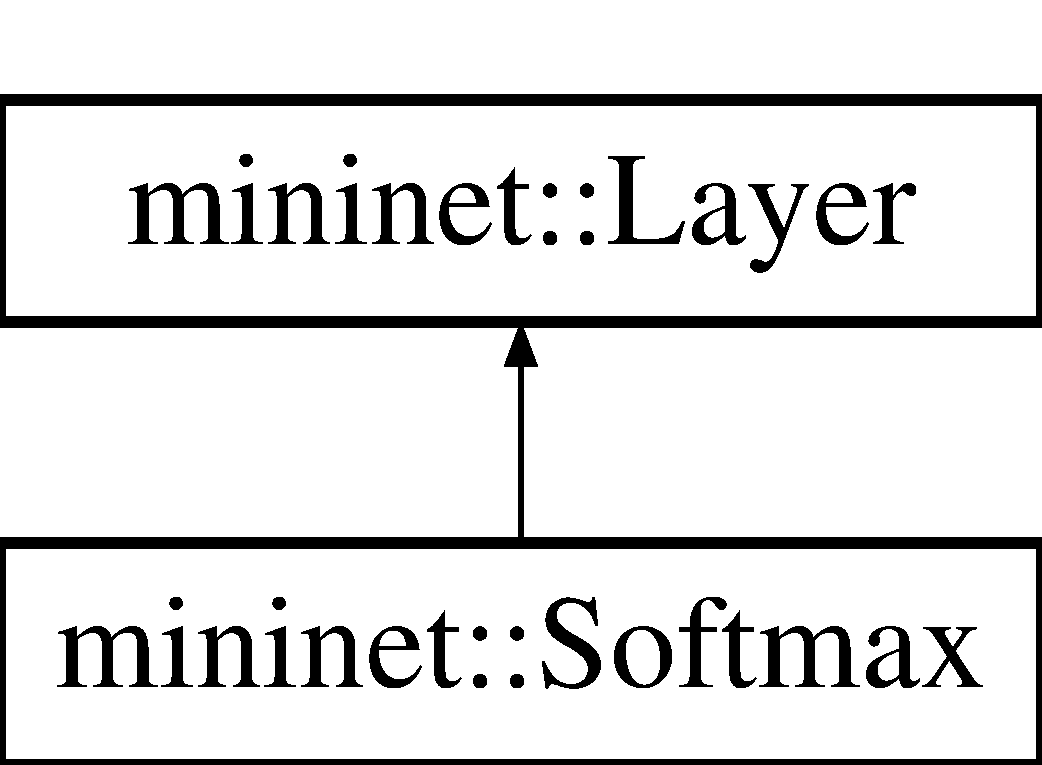
\includegraphics[height=2.000000cm]{classmininet_1_1_softmax}
\end{center}
\end{figure}
\subsection*{Public Member Functions}
\begin{DoxyCompactItemize}
\item 
\hypertarget{classmininet_1_1_softmax_a9305e1361a9da25ed3f528aaeeb20375}{}\label{classmininet_1_1_softmax_a9305e1361a9da25ed3f528aaeeb20375} 
void {\bfseries Forward} (const Vector\+Xd \&input, Vector\+Xd \&output) const
\item 
\hypertarget{classmininet_1_1_softmax_ab4dc8f98bd510e6094efef208a78703c}{}\label{classmininet_1_1_softmax_ab4dc8f98bd510e6094efef208a78703c} 
void {\bfseries Backward} (const Vector\+Xd \&output, const Vector\+Xd \&upstream\+\_\+gammas, Vector\+Xd \&gammas, Vector\+Xd \&deltas) const
\item 
\hypertarget{classmininet_1_1_softmax_a0cbd69a87c7c960989e55ce315aedaa6}{}\label{classmininet_1_1_softmax_a0cbd69a87c7c960989e55ce315aedaa6} 
double {\bfseries Backward} (const Loss\+Functor\+::\+Const\+Ptr \&loss, const Vector\+Xd \&ground\+\_\+truth, const Vector\+Xd \&output, Vector\+Xd \&gammas, Vector\+Xd \&deltas) const
\end{DoxyCompactItemize}
\subsection*{Static Public Member Functions}
\begin{DoxyCompactItemize}
\item 
\hypertarget{classmininet_1_1_softmax_a8d429f52243b6c42e1fb4caec288ede4}{}\label{classmininet_1_1_softmax_a8d429f52243b6c42e1fb4caec288ede4} 
static Layer\+::\+Ptr {\bfseries Create} (size\+\_\+t input\+\_\+size, size\+\_\+t output\+\_\+size)
\end{DoxyCompactItemize}
\subsection*{Additional Inherited Members}


\subsection{Detailed Description}


Definition at line 52 of file softmax.\+h.



The documentation for this class was generated from the following files\+:\begin{DoxyCompactItemize}
\item 
/\+Users/davidfridovichkeil/\+Documents/\+Developer/mininet/include/layer/softmax.\+h\item 
/\+Users/davidfridovichkeil/\+Documents/\+Developer/mininet/src/layer/softmax.\+cpp\end{DoxyCompactItemize}

\hypertarget{classmininet_1_1_trainer}{}\section{mininet\+:\+:Trainer Class Reference}
\label{classmininet_1_1_trainer}\index{mininet\+::\+Trainer@{mininet\+::\+Trainer}}
Inheritance diagram for mininet\+:\+:Trainer\+:\begin{figure}[H]
\begin{center}
\leavevmode
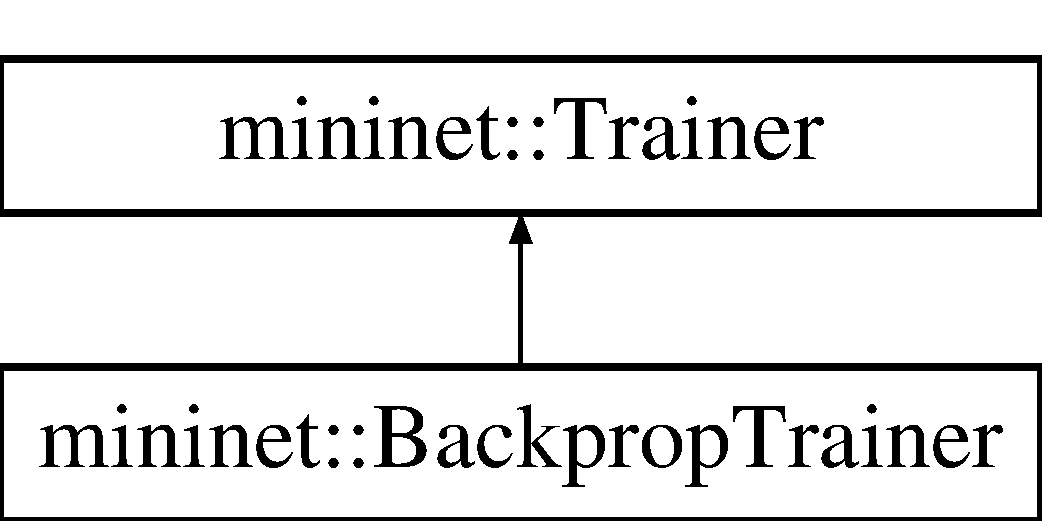
\includegraphics[height=2.000000cm]{classmininet_1_1_trainer}
\end{center}
\end{figure}
\subsection*{Public Member Functions}
\begin{DoxyCompactItemize}
\item 
\hypertarget{classmininet_1_1_trainer_a10eb9b167eec0d9d62ed4441b8addf76}{}\label{classmininet_1_1_trainer_a10eb9b167eec0d9d62ed4441b8addf76} 
{\bfseries Trainer} (const \hyperlink{classmininet_1_1_network}{Network} \&network, const \hyperlink{classmininet_1_1_dataset}{Dataset} \&dataset)
\item 
\hypertarget{classmininet_1_1_trainer_a557fde17a1312e23d3d7d7012c9e2439}{}\label{classmininet_1_1_trainer_a557fde17a1312e23d3d7d7012c9e2439} 
const \hyperlink{classmininet_1_1_network}{Network} \& {\bfseries Immutable\+Network} () const
\item 
\hypertarget{classmininet_1_1_trainer_a2bfdcdf98d5031fe3da6a9a2a48dd986}{}\label{classmininet_1_1_trainer_a2bfdcdf98d5031fe3da6a9a2a48dd986} 
virtual double {\bfseries Train} ()=0
\end{DoxyCompactItemize}
\subsection*{Protected Attributes}
\begin{DoxyCompactItemize}
\item 
\hypertarget{classmininet_1_1_trainer_a7fe0129fba9e72f11ae32e33abc4df12}{}\label{classmininet_1_1_trainer_a7fe0129fba9e72f11ae32e33abc4df12} 
\hyperlink{classmininet_1_1_network}{Network} {\bfseries network\+\_\+}
\item 
\hypertarget{classmininet_1_1_trainer_a18121bfd6966a1b9db98f484b7bf0f2f}{}\label{classmininet_1_1_trainer_a18121bfd6966a1b9db98f484b7bf0f2f} 
\hyperlink{classmininet_1_1_dataset}{Dataset} {\bfseries dataset\+\_\+}
\end{DoxyCompactItemize}


\subsection{Detailed Description}


Definition at line 53 of file trainer.\+h.



The documentation for this class was generated from the following file\+:\begin{DoxyCompactItemize}
\item 
/\+Users/davidfridovichkeil/\+Documents/\+Developer/mininet/include/trainer/trainer.\+h\end{DoxyCompactItemize}

%--- End generated contents ---

% Index
\backmatter
\newpage
\phantomsection
\clearemptydoublepage
\addcontentsline{toc}{chapter}{Index}
\printindex

\end{document}
